\documentclass[tikz]{standalone}
\usepackage{tikz}
\usetikzlibrary{arrows.meta, positioning}
\usepackage[svgnames]{xcolor}
\usepackage{fontspec}
\usepackage{bxcoloremoji}

% Normal distribution approximation (sum of uniform randoms)
\newcommand{\randnormal}[2]{% mean, stddev
  \pgfmathsetmacro{\tmpsum}{(rand+rand+rand+rand+rand+rand)/6}% Range: -1 to 1, approximately normal with stddev sqrt(2)/6
  \pgfmathsetmacro{\result}{#1 + #2 * \tmpsum * 6/sqrt(2)}% Scale to actual stddev
}

% Colors and styles
\definecolor{panelfill}{RGB}{248,248,250}
\definecolor{panelstroke}{RGB}{200,200,210}
\definecolor{ferrospin}{RGB}{213,122,31}
\definecolor{paraspin}{RGB}{70,130,180}
\definecolor{macrobox}{RGB}{240,240,245}

\tikzset{
  spin/.style={line width=1.4pt, -{Stealth[length=6pt]}},
  zoomarrow/.style={line width=1.8pt, -{Stealth[length=16pt, width=10pt]}, draw=black!60, double distance=2pt}
}

\newcommand{\spin}[4]{% x, y, angle, color
  \draw[#4, line width=1pt, fill=#4!12] (#1,#2) circle (0.33);
  \draw[spin,#4] (#1,#2) -- ++({#3}:0.55);
}

\begin{document}
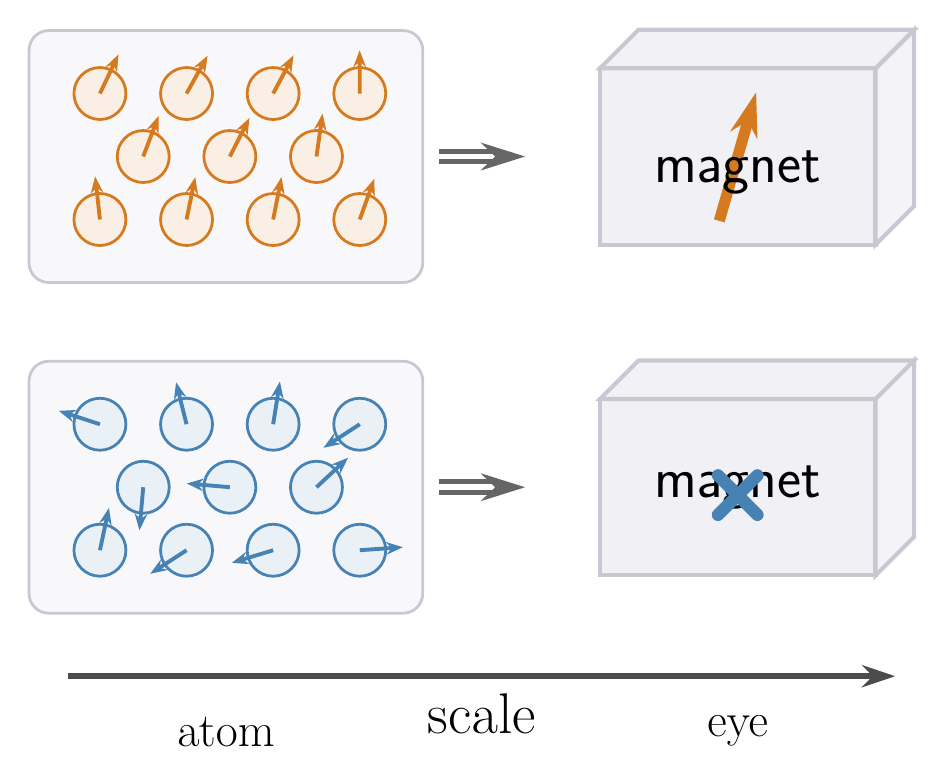
\begin{tikzpicture}[font=\sffamily]
  % Geometry
  \def\panelw{5.0}
  \def\panelh{3.2}
  \def\hgap{1.5}
  \def\vgap{1.0}
  \def\round{0.25}
  
  % Panel positions
  \coordinate (UL) at (0, \panelh+\vgap);
  \coordinate (LL) at (0, 0);
  \coordinate (UR) at (\panelw+\hgap, \panelh+\vgap);
  \coordinate (LR) at (\panelw+\hgap, 0);

  % Upper Left: Ferromagnetic (aligned spins)
  \begin{scope}[shift={(UL)}]
    \filldraw[panelfill, draw=panelstroke, line width=1pt, rounded corners=\round cm]
      (0,0) rectangle (\panelw,\panelh);
    
    % Aligned spins with fluctuation around 74° - programmatically generated
    \pgfmathsetseed{1234}
    \foreach \x in {0.9, 2.0, 3.1, 4.2} {
      \randnormal{74}{15}
      \spin{\x}{2.4}{\result}{ferrospin}
    }
    \foreach \x in {1.45, 2.55, 3.65} {
      \randnormal{74}{15}
      \spin{\x}{1.6}{\result}{ferrospin}
    }
    \foreach \x in {0.9, 2.0, 3.1, 4.2} {
      \randnormal{74}{15}
      \spin{\x}{0.8}{\result}{ferrospin}
    }
  \end{scope}

  % Lower Left: Paramagnetic (random spins)
  \begin{scope}[shift={(LL)}]
    \filldraw[panelfill, draw=panelstroke, line width=1pt, rounded corners=\round cm]
      (0,0) rectangle (\panelw,\panelh);
    
    % Random spins (paramagnetic) - programmatically generated
    \pgfmathsetseed{42} % Set seed for reproducibility
    \foreach \x in {0.9, 2.0, 3.1, 4.2} {
      \pgfmathsetmacro{\randangle}{random(0,359)}
      \spin{\x}{2.4}{\randangle}{paraspin}
    }
    \foreach \x in {1.45, 2.55, 3.65} {
      \pgfmathsetmacro{\randangle}{random(0,359)}
      \spin{\x}{1.6}{\randangle}{paraspin}
    }
    \foreach \x in {0.9, 2.0, 3.1, 4.2} {
      \pgfmathsetmacro{\randangle}{random(0,359)}
      \spin{\x}{0.8}{\randangle}{paraspin}
    }
  \end{scope}

  % Upper Right: Macroscopic magnetization (ferromagnetic phase)
  \begin{scope}[shift={(UR)}]
    % 3D parallelepiped (70% of original size, centered)
    \pgfmathsetmacro{\pw}{3.5}
    \pgfmathsetmacro{\ph}{2.24}
    \pgfmathsetmacro{\depthval}{0.49}
    \pgfmathsetmacro{\offsetx}{(\panelw - \pw) / 2}
    \pgfmathsetmacro{\offsety}{\panelh / 2 - \ph / 2}
    \filldraw[macrobox, draw=panelstroke, line width=1.5pt]
      (\offsetx,\offsety) -- (\offsetx + \pw,\offsety) -- (\offsetx + \pw,\offsety + \ph) -- (\offsetx,\offsety + \ph) -- cycle;
    \filldraw[macrobox!70, draw=panelstroke, line width=1.5pt]
      (\offsetx + \pw,\offsety) -- ++(\depthval,\depthval) -- ++(0,\ph) -- ++(-\depthval,-\depthval) -- cycle;
    \filldraw[macrobox!85, draw=panelstroke, line width=1.5pt]
      (\offsetx,\offsety + \ph) -- (\offsetx + \pw,\offsety + \ph) -- ++(\depthval,\depthval) -- ++(-\pw,0) -- cycle;
    
    % Enhanced magnetization arrow with magnet emoji at center
    \pgfmathsetmacro{\arrowx}{\offsetx + \pw/2}
    \pgfmathsetmacro{\arrowy}{\offsety + \ph/2}
    \pgfmathsetmacro{\arrowangle}{74}  % Direction of magnetization
    \pgfmathsetmacro{\arrowlength}{1.7}  % Total length
    \draw[ferrospin, line width=4pt, -{Stealth[length=16pt, width=10pt]}] 
      (\arrowx, \arrowy) ++ (\arrowangle+180:\arrowlength/2) -- ++(\arrowangle:\arrowlength);
    \node[yshift=-2mm] at (\arrowx, \arrowy) {\huge \coloremojicode{magnet}};
  \end{scope}

  % Lower Right: No magnetization (paramagnetic phase)
  \begin{scope}[shift={(LR)}]
    % 3D parallelepiped (70% of original size, centered)
    \pgfmathsetmacro{\pw}{3.5}
    \pgfmathsetmacro{\ph}{2.24}
    \pgfmathsetmacro{\depthval}{0.49}
    \pgfmathsetmacro{\offsetx}{(\panelw - \pw) / 2}
    \pgfmathsetmacro{\offsety}{\panelh / 2 - \ph / 2}
    \filldraw[macrobox, draw=panelstroke, line width=1.5pt]
      (\offsetx,\offsety) -- (\offsetx + \pw,\offsety) -- (\offsetx + \pw,\offsety + \ph) -- (\offsetx,\offsety + \ph) -- cycle;
    \filldraw[macrobox!70, draw=panelstroke, line width=1.5pt]
      (\offsetx + \pw,\offsety) -- ++(\depthval,\depthval) -- ++(0,\ph) -- ++(-\depthval,-\depthval) -- cycle;
    \filldraw[macrobox!85, draw=panelstroke, line width=1.5pt]
      (\offsetx,\offsety + \ph) -- (\offsetx + \pw,\offsety + \ph) -- ++(\depthval,\depthval) -- ++(-\pw,0) -- cycle;
    
    % No magnetization - magnet emoji with blue X overlay
    \pgfmathsetmacro{\centerx}{\offsetx + \pw/2}
    \pgfmathsetmacro{\centery}{\offsety + \ph/2}
    \pgfmathsetmacro{\crosswidth}{4.5}  % Tunable cross line width
    \node[] at (\centerx, \centery) {\huge \coloremojicode{magnet}};
    \draw[paraspin, line width=\crosswidth pt, line cap=round] 
      (\centerx - 0.25, \centery - 0.35) -- (\centerx + 0.25, \centery + 0.15);
    \draw[paraspin, line width=\crosswidth pt, line cap=round] 
      (\centerx - 0.25, \centery + 0.15) -- (\centerx + 0.25, \centery - 0.35);
  \end{scope}

  % Zoom arrows (RG flow style)
  % Upper row: from ferromagnetic microscopic to macroscopic
  \draw[zoomarrow] ([xshift=0.2cm]UL) ++ (\panelw, \panelh/2) -- ++(\hgap-0.4, 0);
  
  % Lower row: from paramagnetic microscopic to macroscopic
  \draw[zoomarrow] ([xshift=0.2cm]LL) ++ (\panelw, \panelh/2) -- ++(\hgap-0.4, 0);

  % Scale arrow at bottom
  \draw[line width=2pt, -{Stealth[length=12pt, width=8pt]}, draw=black!70] 
    (0.5, -0.8) -- (\panelw+\hgap+\panelw-0.5, -0.8)
    node[midway, below=2pt, font=\large] {\huge scale};

  % Emojis below scale arrow
  % Microscope emoji at left panel center (representing microscopic scale)
  \node[font=\Large] at (\panelw/2, -1.5) {\LARGE\coloremojicode{atom}};
  % Eye emoji at right panel center (representing macroscopic/observable scale)
  \node[font=\Large] at (\panelw+\hgap+\panelw/2, -1.5) {\LARGE\coloremojicode{eye}};

\end{tikzpicture}
\end{document}
